\documentclass [tikz] {standalone}
\begin{document}    
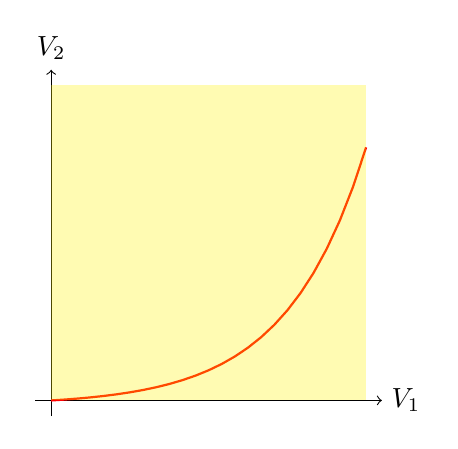
\begin{tikzpicture}[domain=0:4]

    \draw[->] (-0.2,0) -- (4.2,0) node[right] {$V_1$};
    \draw[->] (0,-0.2) -- (0,4.2) node[above] {$V_2$};
    \draw[color=red, thick] plot (\x,{0.06*exp(\x) - 0.06});
    \fill[yellow, fill opacity = 0.3] (0,0)   rectangle (4,4);

\end{tikzpicture}

\end{document}